\section{Introduction}
% 
\acrfull{acs} plays a crucial role in every enterprise. They are used for the physical access to company premises, online, and internal resources. There are countless of different systems and providers, with offerings ranging from simple access-card-based systems, password-based log-in screens to complex systems combining different types of physical and online access to resources. 

The problem of today’s access systems is that they are usually handling physical and online accesses separately. Two systems must be implemented and maintained, and companies usually only specialise in providing one of those systems. Companies such as HID\footnote{\url{https://www.hidglobal.com/solutions/access-control-systems}, accessed 26 March 2019} or G4S\footnote{\url{https://www.g4s.com/en-gb/what-we-do/security-services/fire-and-security-systems/symmetry-software}, accessed 26 March 2019} are providing physical \acrshort{acs} to enterprises which allows employees to access the building, rooms, canteen, or garage, based on their access level. On the other side of the spectrum, there are tech companies such as Microsoft\footnote{\url{https://docs.microsoft.com/en-us/windows-server/identity/ad-ds/get-started/virtual-dc/active-directory-domain-services-overview}, accessed 26 March 2019} which offer software for managing employees’ access to online services and resources.

Therefore, there exist two mostly independent systems intended for similar use cases. These systems are either managed individually or can be interconnected, so that there is one endpoint for managing accesses. Both approaches work fine, but what if there was an \acrshort{acs} which would combine both physical and online access? What if physical access would be possible by authenticating the employee with a smartcard, smartphone or an authenticator key? Simply, there would only be a need for one device, with which an employee would be able to access premises, as well as authenticate themselves when logging-in to an online service. Such a system does not only solve the problem of the employees’ experience and convenience of having to carry around an access card, but also a problem of security of the corporate account caused by passwords. The reason is that many companies have policies that require a change of password every few months and therefore, employees tend to use easy to remember passwords. Furthermore, many corporate accounts have been compromised by phishing attacks\cite{Kessem2017CanadianAttacks}. This can be avoided by using physical authenticators instead of passwords.

The aim of this project is to address this problem and propose a system, where physical access control and online access control is managed from a single system. Another very important feature introduced by this system, is the possibility of using \acrshort{fido}2 authenticator with \acrshort{nfc}, or a smartphone to access a building, rooms or printers. Both devices would work similarly to an access card which is usually given to an employee on their first day. It is common these days, that employees sign in to many online services with their corporate account. To avoid passwords, \acrshort{fido}2 can be used for authentication when logging in to an account, by using an authenticator -- either a physical key device or a smartphone. This allows for \textit{strong authentication}~\cite{McDowell2017WhyAlliance}. The only thing the employee needs to type in during logging in is their user ID. They are afterwards authenticated, if they can demonstrate the possession of their \acrshort{fido}2 authenticator. The access card is therefore replaced by an authenticator (which can also be smartphone-based) and the employee does no longer need to remember a password.

Secondary aim of this system lies in the access management, which grants or denies the entry or use of a service for an employee. To facilitate this, policies, attributes or role-based access can be implemented, which enable automated, fine-grained access control.

% assigning to each employee a role/s and  attributes or creating policies by which the access will be granted or denied automatically.

% \begin{figure}[ht]
%     \centering
%     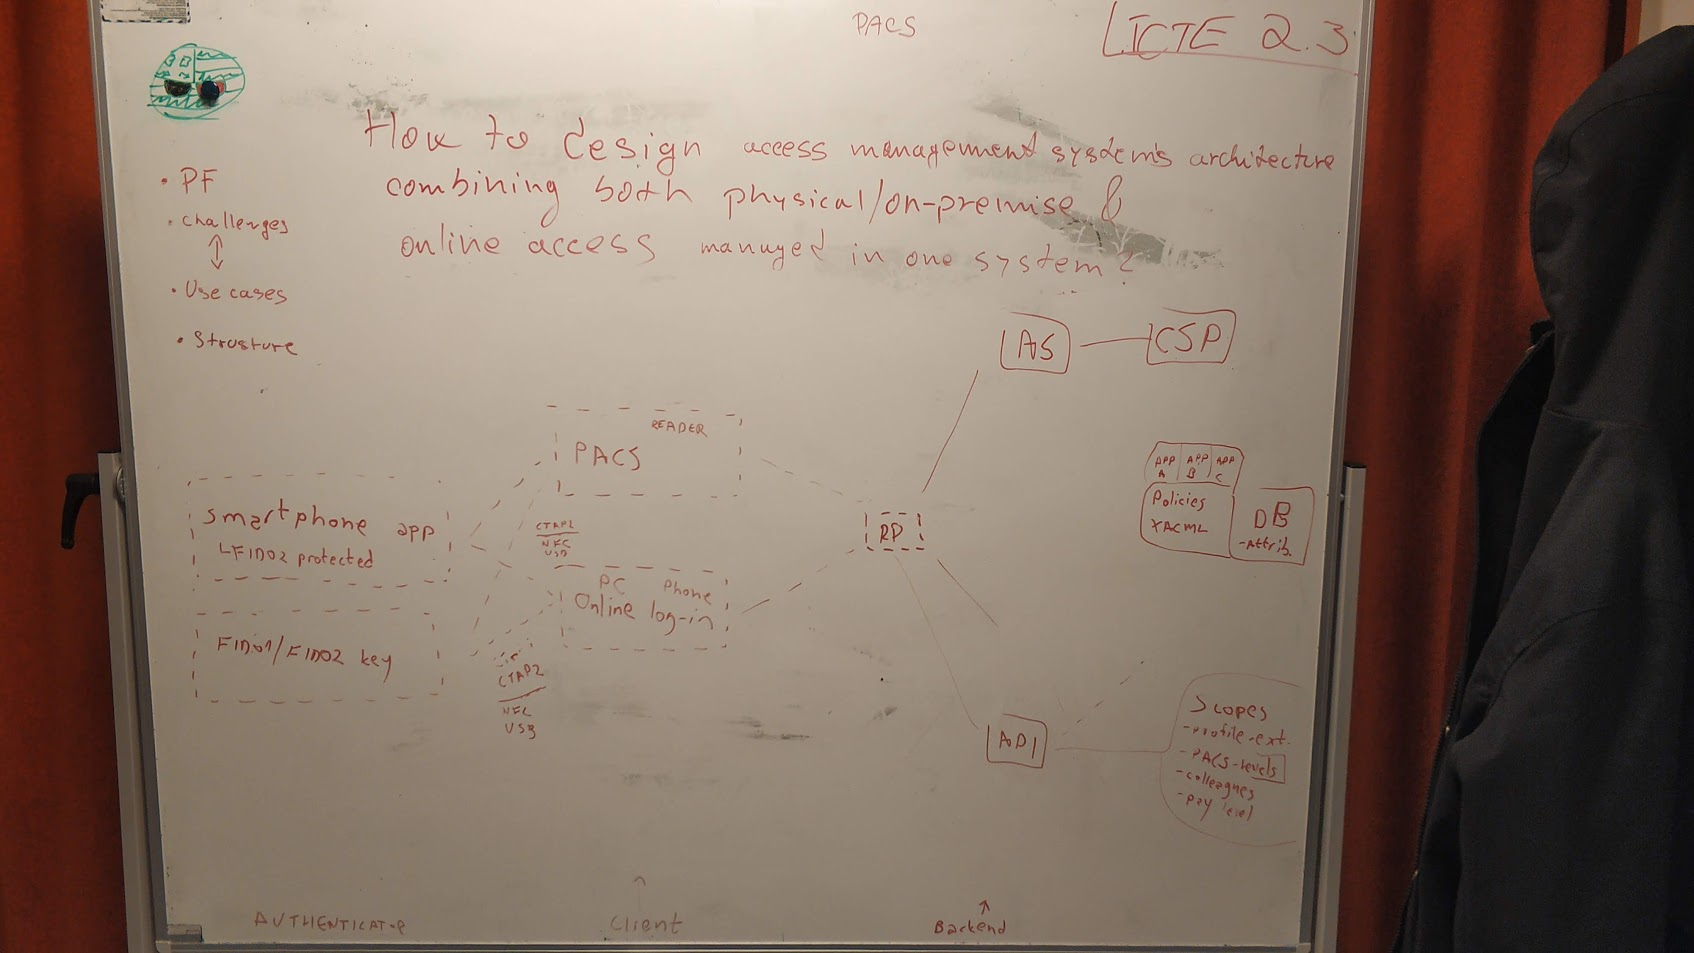
\includegraphics[width=.95\textwidth]{00images/IntroArchitecture}
%     \caption{Explanation! + new diagram}
%     \label{fig:IntroArchitecture}
% \end{figure}

\subsection{Challenges} \label{challenges}

There is a number of challenges, which the current \acrshort{acs} in enterprises are facing. One of the major concerns of every access system is its security. Passwords are often targeted as the weakest link in the system. Every employee has their corporate account linked with many services and is accessing many protected resources. Often employees are forced to change their passwords periodically. Therefore, choosing a weak password and successful phishing attacks are a threat which can be solved by two-factor authentication, but as showed in \acrshort{nist} Special Publication 800-63B \cite{Grassi2017DigitalManagement} there are threats still associated with \acrshort{mfa} such as Social engineering, Phishing attacks or Endpoint compromise. Choosing a right combination of factors for authentication is therefore crucial.

Living in the era of fast technical advance, employees also require convenience when using access systems and carrying around an access card is not the most convenient method anymore, as shown in study by HID~\cite{2017AccessGlobal}, where 61\% of respondents sees integration between systems as hugely beneficial for user convenience or by Netflix~\cite{2012NetflixPilot}, where 87.5\% of respondents would like to use smartphones to open doors in the workplace for authentication. \acrshort{acs} should therefore, offer more convenient ways of authentication -- for example a smartphone.

Often, the physical access control and access policy management systems are two separate entities in enterprises. This requires more resources spend on managing these systems, as well as more set-up work when a new employee is hired or leaves the company. Having one system to handle these tasks is thus desirable.
\subsection{Problem formulation} \label{problemFormulation}
The motivation for this project comes from the existing split of online and physical access control systems. Secondary, the low security of passwords has been demonstrated by several phishing cases and their use is discouraged.
% TODO add reference here
Alternative ways of strong authentication have been proposed instead, including physical cryptographic devices.
% TODO add reference here
The banking industry, which has been using similar tokens for a long period of time already (credit cards), has now witnessed the migration of these tokens to smartphones, mainly for user convenience.
% TODO add reference here
Such migration is also technically possible in access control scenarios, although its use has been limited in practice.

Taking into account the challenges and issues mentioned previously, we propose an innovative \acrshort{acs} that addresses these issues, by building on top of state-of-the-art technologies in the field. The problem formulation is as follows:

\begin{center}
    \textit{“How to design an Access control system, combining both physical and online access control, that includes strong authentication and enables the use of smartphone?”}
\end{center}

\paragraph{Sub-questions}
We define the following sub-problems to help guide us in the analysis and design of the system:

% TODO Is this still draft?
\begin{itemize}[noitemsep]
    \item What solutions are there on the market?
    \item What is the system architecture?
    \item Which technologies are the best for proposed system?
    \item Which components of the system must be implemented for MVP?
    \item What are the requirements of the system?
\end{itemize}
\subsection{Report Structure}

